\section{Method}
\label{sec:method}

\begin{figure*}[t]
    \centering
    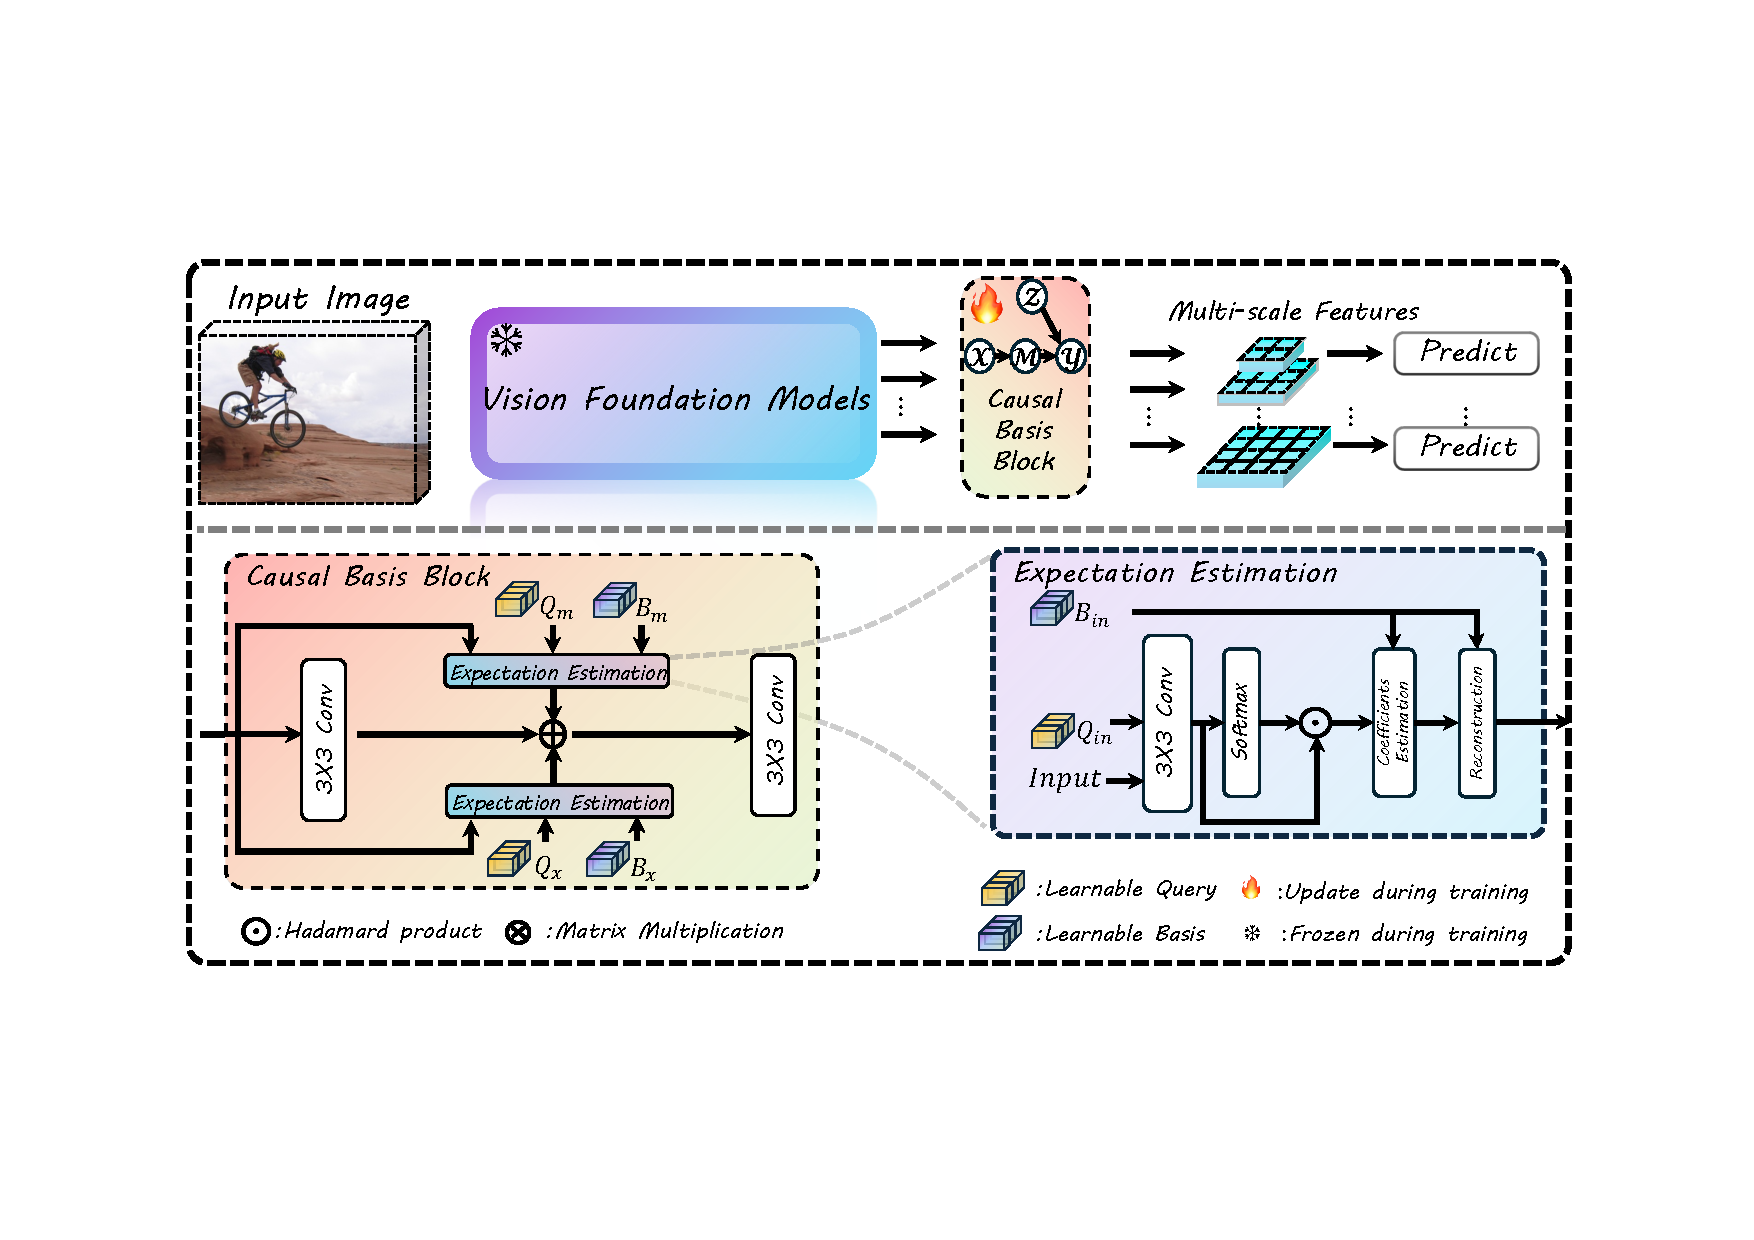
\includegraphics[width=1.0\textwidth]{figs/pipev2.pdf}
    % \caption{Overview of the proposed \textbf{\textit{Bridge}}. Multi-scale features are first extracted from the Vision Foundation Model, then calibrated using Causal Basis Blocks，and finally fed into task-specific heads for prediction.}
    \caption{Overview of the proposed \textbf{\textit{Bridge}}. Multi-scale features are first extracted from the Vision Foundation Model, then calibrated using the Causal Basis Block (CBB). Within the CBB, the Coefficients Estimation and Reconstruction components in Expectation Estimation refer to Equation~\ref{equ:coefficients} and Equation~\ref{equ:expected_reconstruction}, respectively. The calibrated features are finally fed into task-specific heads for prediction.}
    \label{fig:pipe}
\end{figure*}

\subsection{Preliminaries}
\subsubsection{Task Formulation}
In DG tasks, given the source domains $\mathcal{S}=\left\{\mathbf{x}^s, \mathbf{y}^s\right\}$,
the goal is to learn a model $f: \mathcal{X} \rightarrow \mathcal{Y}$ that generalizes well to unseen target domains $\mathcal{T}=\left\{\mathbf{x}^t, \mathbf{y}^t\right\}$.
Here, $\mathcal{X}$ and $\mathcal{Y}$ denote the input and output spaces, respectively.
Note that the marginal distributions of the source and target domains differ (i.e., $\mathcal{P}_{X}^S \neq \mathcal{P}_{X}^T$) mainly due to discrepancies in data sources.
% , which lead to domain-specific variations in object categories, co-occurrence patterns, and stylistic or contextual attributes (e.g., background, illumination, texture, and shape).
% Note that the marginal distributions of the source and target domains differ (i.e., $\mathcal{P}_{X}^S \neq \mathcal{P}_{X}^T$)
% due to domain-specific variations in object categories and their co-occurrence patterns; stylistic and contextual shifts (e.g., background, illumination, texture, and shape); and biases introduced during data sourcing.
\subsubsection{Front-door Adjustment}
% In visual scenes, objects often co-occur with others and exhibit diverse textures and shapes; the former act as observable confounders, whereas the latter are unobservable.
Visual recognition involves various confounding factors, such as background, illumination, texture, and context, which bias the model’s estimation of the underlying relationship between inputs and semantic labels.
To illustrate this effect, by Bayes' rule, we have
\begin{equation}
    \mathcal{P}(\mathcal{Y} \mid \mathcal{X}) 
    = \sum_{\mathcal{Z}} \mathcal{P}(\mathcal{Y} \mid \mathcal{X}, \mathcal{Z}) \, \mathcal{P}(\mathcal{Z} \mid \mathcal{X}),
    \label{equ:bayes_rule}
\end{equation}
where $\mathcal{Z}$ denotes confounders, which induce spurious correlations between $\mathcal{X}$ and $\mathcal{Y}$ via $\mathcal{P}(\mathcal{Z}\mid\mathcal{X})$.
Note that $\mathcal{P}(\mathcal{Z}\mid\mathcal{X})$ may \textbf{dominate} the prediction of the model when samples are limited, leading the model to rely on spurious correlations rather than causal features (Please refer to supplementary material for the explanation).
To block the back-door paths $\mathcal{Z} \cancel{\to} \mathcal{X} \to \mathcal{Y}$, the back-door adjustment using the do operator~\cite{pearl2018book} conditions on $\mathcal{Z}$ as follows:
\begin{equation}
    \mathcal{P}(\mathcal{Y} \mid \mathrm{do}(\mathcal{X})) 
    = \sum_{\mathcal{Z}} \mathcal{P}(\mathcal{Y} \mid \mathcal{X}, \mathcal{Z}) \, \mathcal{P}(\mathcal{Z}).
    \label{equ:back_door_adjustment}
\end{equation}




However, in practice, some confounders $\mathcal{Z}$ may be unobserved or difficult to measure, 
making such an adjustment infeasible.
Fortunately, front-door adjustment provides a principled way to mitigate such spurious correlation effects 
without explicitly modeling the confounders.
Specifically, a mediator variable $\mathcal{M}$ is introduced on the causal path from $\mathcal{X}$ to $\mathcal{Y}$. 
This mediator can block the spurious correlation path from $\mathcal{Z}$ to $\mathcal{X}$.
Mathematically, the front-door adjustment is formulated as follows:
\begin{equation}
\resizebox{0.433\textwidth}{!}{%
$\displaystyle
\begin{aligned}
\mathcal{P}(\mathcal{Y} \mid \mathrm{do}(\mathcal{X})) 
&= \sum_{\mathcal{M}} \mathcal{P}(\mathcal{Y} \mid \mathcal{M}, \mathrm{do}(\mathcal{X})) 
   \, \mathcal{P}(\mathcal{M} \mid \mathrm{do}(\mathcal{X})) \\
&= \sum_{\mathcal{M}} \mathcal{P}(\mathcal{M} \mid \mathcal{X}) 
   \sum_{\mathcal{X}'} \mathcal{P}(\mathcal{Y} \mid \mathcal{X}', \mathcal{M}) \, \mathcal{P}(\mathcal{X}') \\
&= \mathbb{E}_{\mathcal{M} \sim \mathcal{P}(\mathcal{M} \mid \mathcal{X})} 
   \Big[ \, \mathbb{E}_{\mathcal{X}' \sim \mathcal{P}(\mathcal{X})} 
        [\, \mathcal{P}(\mathcal{Y} \mid \mathcal{X}', \mathcal{M}) \,] 
   \Big],
\end{aligned}%
$}
\label{equ:front_door_adjustment}
\end{equation}
where $\mathcal{X}'$ denotes potential inputs sampled from the entire input space, distinct from the observed $\mathcal{X}$.

Recently, Wang et al.~\cite{wang2024vision} extended the front-door adjustment from the network's final prediction layer 
to intermediate feature layers, formulating it as a linear mapping model.
Accordingly, Equation~\ref{equ:front_door_adjustment} can be reformulated as:
\begin{equation}
\mathcal{P}(\mathcal{Y} \mid \mathrm{do}(\mathcal{X}))
= \mathbb{E}_{\mathcal{M} \sim \mathcal{P}(\mathcal{M} \mid \mathcal{X})}[\mathcal{M}] 
   + \mathbb{E}_{\mathcal{X}' \sim \mathcal{P}(\mathcal{X})}[\mathcal{X}'].
\label{equ:front_door_adjustment_linear}
\end{equation}

Thus, implementing the front-door adjustment reduces to estimating the two expectations 
$\mathbb{E}_{\mathcal{M} \mid \mathcal{X}}[\mathcal{M}]$ and $\mathbb{E}_{\mathcal{X}'}[\mathcal{X}']$.

\subsection{Overview}
This section presents \textbf{\textit{Bridge}}, a DGOD method built on VFMs. \textbf{\textit{Bridge}} applies front-door adjustment to VFMs' features through the basis learning mechanism, producing causal and robust representations for downstream tasks.
Figure~\ref{fig:pipe} illustrates the overall architecture of \textbf{\textit{Bridge}}. Specifically, given an input image, multi-scale feature maps are first extracted using the VFMs, then refined through the proposed Causal Basis Block to improve robustness and generalization.
The resulting calibrated features are finally passed to task-specific heads for prediction.
\subsection{Causal Basis Block}
Inspired by dictionary learning~\cite{tovsic2011dictionary}, in which data are represented as combinations of basis vectors, 
we approximate the expectations in Equation~\ref{equ:front_door_adjustment_linear} 
as linear combinations of learnable basis vectors:
\begin{equation}
    \mathbb{E}[\mathcal{V}] \approx \frac{1}{S} \sum_{i=1}^S \sum_{k=1}^K c_{ik} b_k,
    \label{equ:expectation_basis_avg}
\end{equation}
where $\mathcal{V}$ denotes a generic variable (e.g., $\mathcal{M}\mid\mathcal{X}$ or $\mathcal{X}'$), 
$b_k$ ($k=1,\dots,K$) are the learnable basis vectors, 
$S$ is the total number of samples, and $c_{ik}$ are the coefficients for each sample.

\subsubsection{Expectations Estimation} 
\label{sec:coefficients_estimation}
To implement Equation~\ref{equ:expectation_basis_avg}, we describe how the basis vectors and their coefficients are learned.
We design a module termed the \textbf{Causal Basis Block} (CBB), which jointly estimates coefficients and learns bases in an end-to-end differentiable manner.

Given input feature maps $\mathcal{X}_\mathrm{in} \in \mathbb{R}^{B \times N \times C}$ (where $N = H \times W$, with $H$ and $W$ denoting the height and width), the CBB introduces a set of learnable \textit{Sample Queries}
$\mathcal{Q}_s \in \mathbb{R}^{1 \times S \times C}$, which act similarly to the 
\textit{object queries} in DETR~\cite{carion2020end} and Mask2Former~\cite{cheng2022masked}.
During training, these queries implicitly aggregate global representations from the training set, guiding the estimation of expectations.

First, the \textit{Sample Queries} interact with the input features to produce multiple correlation maps, which are then aggregated through a weighted operation:
\begin{equation}
\resizebox{0.433\textwidth}{!}{%
$\displaystyle
   \mathcal{A} \;=\;
   \sum_{i=1}^{S}
   (\mathcal{Q}_s \mathcal{X}_\mathrm{in})_i
   \odot
   \operatorname{Softmax}((\mathcal{Q}_s \mathcal{X}_\mathrm{in}))_i
   \in \mathbb{R}^{B \times N \times 1},
   \label{equ:avg_correlation_corrected}
   $}
\end{equation}
where \(\mathcal{A}\) is an expected spatial weighting map and \(\odot\) denotes element-wise multiplication.

We then obtain a query-guided representation by reweighting the input features with $\mathcal{A}$:
\begin{equation}
    \mathcal{X}_{q} = \mathcal{A}  \odot \mathcal{X}_\mathrm{in} \in \mathbb{R}^{B \times N \times C},
    \label{equ:query_aggregation}
\end{equation}
where $\mathcal{X}_{q}$ emphasizes the generalized information of the input $\mathcal{X}_\mathrm{in}$
by reweighting it with the expected spatial weighting map.

With the query-guided features $\mathcal{X}_{q}$, we introduce a set of learnable bases
$\mathcal{B} = [b_1, \dots, b_K] \in \mathbb{R}^{K \times C}$ ($K < C$), providing a low-rank subspace for representation.
Projecting $\mathcal{X}_{q}$ onto this subspace enables reconstruction with fewer bases while preserving the most representative components. The coefficients $\mathcal{C}$ of $\mathcal{X}_{q}$ w.r.t.\ $\mathcal{B}$ are computed as:
\begin{equation}
   \mathcal{C} = (\mathcal{B}^{\top} \mathcal{B})^{-1} \mathcal{B}^{\top} \mathcal{X}_{q}
   \in \mathbb{R}^{B \times N \times K},
   \label{equ:coefficients}
\end{equation}
where $(\mathcal{B}^{\top} \mathcal{B})^{-1}$ denotes a normalization term since the bases may not remain orthogonal during training.

By first reweighting with $\mathcal{A}$ to highlight generalizable information and then projecting onto the low-rank subspace to remove redundancy, the estimated coefficients $\mathcal{C}$ are encouraged to approximate $\frac{1}{S}\sum_{i=1}^S\sum_{k=1}^K c_{ik}$, capturing the intrinsic representation aggregated by the \textit{Sample Queries} and filtered through the subspace projection.
We finally estimate the expectation in Equation~\ref{equ:expectation_basis_avg} as:
\begin{equation}
\mathbb{E}[\mathcal{X}_\mathrm{in}] \approx \mathcal{C} \mathcal{B}\ \in \mathbb{R}^{B \times N \times C}.
\label{equ:expected_reconstruction}
\end{equation}

In summary, since closed-form expectations in complex representation spaces are intractable, 
we employ \textit{Sample Queries} and subspace projection to approximate them: the queries aggregate generalizable cross-sample information, and the projection filters it into a low-rank space spanned by $\mathcal{B}$, rejecting redundancy while preserving representative structure (illustratively: $\mathbb{R}^{N \times C} \to \mathbb{R}^{N \times K} \to \mathbb{R}^{N \times C}$).
The low-rank, learnable bases naturally capture the principal modes of the feature space, and this compression effectively aligns features with the core directions of the sample distribution, thereby approximating the sample expectation.

Note that the entire procedure is \textbf{differentiable} and can be optimized end-to-end with the network.
At inference, the term $\mathcal{B} (\mathcal{B}^{\top} \mathcal{B})^{-1} \mathcal{B}^{\top}$ can be precomputed and absorbed into a single $C \times C$ matrix, reducing computation and simplifying deployment.


\subsubsection{Feature Aggregation}
CBB outputs a combination of expected features and mediator features, capturing both generalized and task-specific information.  
First, the mediator features $\mathcal{M}$ are computed by applying a simple convolutional block to the input features $\mathcal{X}$:  
\begin{equation}
   \mathcal{M} = \mathrm{Conv}(\mathcal{X}).
\end{equation}

We then estimate the expectations $\hat{\mathbb{E}}[\mathcal{X}]$ (ideally, $\mathbb{E}[\mathcal{X}'] = \mathbb{E}[\mathcal{X}])$ and $\hat{\mathbb{E}}[\mathcal{M}]$ 
using the coefficient estimation method described in Sec.~\ref{sec:coefficients_estimation}. 
The final output is obtained by combining these estimates with the mediator features:

\begin{equation}
   \mathcal{F}_{\text{out}} = \hat{\mathbb{E}}[\mathcal{X}] + \hat{\mathbb{E}}[\mathcal{M}] + \mathcal{M}.
\end{equation}

The first two terms implement the front-door adjustment, mitigating spurious correlations, while the inclusion of $\mathcal{M}$ preserves task-specific information for downstream processing. Note that the CBB is trained end-to-end using the downstream task loss, with no additional supervision required.





% What about the loss functions?
